% LaTeX source for ``Think Complexity, 2nd edition''
% Copyright (c)  2016  Allen B. Downey.

% Permission is granted to copy, distribute, transmit and adapt
% this work under a Creative Commons
% Attribution-NonCommercial-ShareAlike 4.0 International (CC BY-NC-SA 4.0)
% https://creativecommons.org/licenses/by-nc-sa/4.0/

% If you are interested in distributing a commercial version of this
% work, please contact Allen Downey.

% The LaTeX source for this book is available from
% http://greenteapress.com/complexity


\documentclass[12pt]{book}

\begin{document}

\chapter{Evolution}

The most important idea in biology, and possibly all of science, is the {\bf theory of evolution by natural selection}, which claims that new species are created, and existing species change over time, due to natural selection.  Natural selection is a process in which heritable differences between individuals cause differences in survival or reproduction (or both).

Among people who know something about biology, the theory of evolution is widely regarded as a fact, which is to say that it close enough to the truth that if it is corrected in the future, the amendments will leave the central ideas substantially intact.

Nevertheless, many people do not believe in evolution.  In a survey run by the Pew Research Center, survey respondents were asked which of the following claims is closer to their view:

\begin{enumerate}

\item Humans and other living things have evolved over time.

\item Humans and other living things have existed in their present form since the beginning of time.

\end{enumerate}

About 34\% of Americans chose the second (\see \url{http://www.thearda.com/Archive/Files/Codebooks/RELLAND14_CB.asp}).

Even among the ones who believe that living things have evolved, barely more than half believe that the cause of evolution is natural selection.  In other words, only about 33\% of Americans believe that the theory of evolution is true.

How is this possible?  In my opinion, contributing factors include:

\begin{itemize}

\item Some people think that there is a conflict between evolution and their religious beliefs and, feeling like they have to reject one, they reject evolution.

\item Others have been actively misinformed, often by members of the first group, so that much of what they know about evolution is false.

\item And many people simply don't know anything about evolution.

\end{itemize}

There's probably not much I can do about the first group, but I think I can help the others.  Empirically, the theory of evolution is hard for people to understand.  At the same time, it is profoundly simple: for many people, once they understand it, it seems both obvious and irrefutable.

To help people make this transition from confusion to clarity, the most powerful tool I have found is computation.  Ideas that are hard to understand in theory can be easy to understand when we see them happening in simulation.  
That is the goal of this chapter.

%TODO: The code for...

\section{Simulating evolution}

I will start with a simple model that demonstrates a basic form of evolution.  According to the theory, the following features are sufficient to produce evolution:

\begin{itemize}

\item Replicators:  We need a population of agents that can reproduce in some way.  We'll start with replicators that make perfect copies of themselves.  Later we'll add imperfect copying, that is, mutation.

\item Variation:  We also need some variability in the population, that is, differences between individuals.

\item Differential survival or reproduction:  The differences between individuals have to affect their ability to survive or reproduce.

\end{itemize}

To simulate these features, we'll define a population of {\bf agents} that represent individual organisms.  Each agent has genetic information, called its {\bf genotype}, which is the information that gets copied when the agent replicates.  In our model, a genotype is represented by a sequence of \py{N} binary digits (zeros and ones), where \py{N} is a parameter we can choose.

To generate a population with variation, we choose initial genotypes at random; later we will explore mechanisms that generate or increase variation.

Finally, to generate differential survival and reproduction, we define a function that maps from each genotype to a {\bf fitness}, where fitness is a quantity related to the ability of an agent to survive or reproduce.

\section{Fitness landscape}

The function that maps from genotype to fitness is called a {\bf fitness landscape}.  In the landscape metaphor, each genotype corresponds to a location in an \py{N}-dimensional space, and fitness corresponds to the ``height" of the landscape at that location.  For visualizations that might clarify this metaphor, see \url{https://en.wikipedia.org/wiki/Fitness_landscape}.

In biological terms, the fitness landscape represents information about how the genotype of an organism is related to its physical form and capabilities, called its {\bf phenotype}, and how the phenotype interacts with its {\bf environment}.

In the real world, fitness landscapes are complicated, but we don't need to build a realistic model.  To induce evolution, we need {\em some} relationship between genotype and fitness, but it turns out that it can be {\em any} relationship.  To demonstrate this point, we'll generate the fitness function at random.

Here is the definition for a class that represents a fitness landscape:

\begin{code}
class FitnessLandscape:
    def __init__(self, N):
        self.N = N
        self.one_values = np.random.random(N)
        self.zero_values = np.random.random(N)
        
    def fitness(self, loc):
        fs = np.where(loc, self.one_values, 
                           self.zero_values)
        return fs.mean()
\end{code}

The genotype of an agent, which corresponds to its location in the fitness landscape, is represented by a NumPy array of zeros and ones, called \py{loc}.
The fitness of a given genotype is the mean of \py{N} {\bf fitness contributions}, one for each element of \py{loc}.

To compute the fitness of a genotype, \py{FitnessLandscape} uses two arrays:
\py{one_values}, which contains the fitness contributions of having a \py{1} in each element of \py{loc}, and \py{zero_values}, which contains the fitness contributions of having a \py{0}.

The \py{fitness} method uses \py{np.where} to select a value from \py{one_values} where \py{loc} has a \py{1}, and a value from \py{zero_values} where \py{loc} has a \py{0}.

As an example, suppose \py{N=3} and

\begin{code}
one_values =  [0.1, 0.2, 0.3]
zero_values = [0.4, 0.7, 0.9]
\end{code}

In that case, the fitness of \py{loc = [0, 1, 0]} would be the mean of \py{[0.4, 0.2, 0.9]}, which is \py{0.5}.


\section{Agents}

Next we need agents.  Here's the class definition:

\begin{code}
class Agent:
    
    def __init__(self, loc, fit_land):
        self.loc = loc
        self.fit_land = fit_land
        self.fitness = fit_land.fitness(self.loc)
        
    def copy(self):
        return Agent(self.loc, self.fit_land)
\end{code}

The attributes of an \py{Agent} are:

\begin{itemize}

\item \py{loc}: The location of the \py{Agent} in the fitness landscape.

\item \py{fit_land}: A reference to a \py{FitnessLandscape} object.

\item \py{fitness}: The fitness of this \py{Agent} in the \py{FitnessLandscape}, represented as a number between 0 and 1.

\end{itemize}

This definition of \py{Agent} provides a simple \py{copy} method that copies the genotype exactly; later, we will see a version that copies with mutation, but mutation is not necessary for evolution.


\section{Simulation}

Now that we have agents and a fitness landscape, I'll define a class called \py{Simulation} that simulates the creation, reproduction, and death of the agents.  To avoid getting bogged down, I'll present a simplified version of the code here; you can see the details in the notebook for this chapter.

Here's the definition of \py{Simulation}:

\begin{code}
class Simulation:
    
    def __init__(self, fit_land, agents):
        self.fit_land = fit_land
        self.agents = agents
\end{code}

The attributes of a \py{Simulation} are:

\begin{itemize}

\item \py{fit_land}: A reference to a \py{FitnessLandscape} object.

\item \py{agents}: An array of \py{Agent} objects.

\end{itemize}

The most important function in \py{Simulation} is \py{step}, which simulates one time step:

\begin{code}
# class Simulation:
    
    def step(self):
        n = len(self.agents)
        fits = self.get_fitnesses()
        
        # see who dies
        index_dead = self.choose_dead(fits)
        num_dead = len(index_dead)
        
        # replace the dead with copies of the living
        replacements = self.choose_replacements(num_dead, fits)
        self.agents[index_dead] = replacements
\end{code}

\py{step} uses three other methods:

\begin{itemize}

\item \py{get_fitnesses} returns an array containing the fitness of each agent in the order they appear in the agent array.

\item \py{choose_dead} decides which agents die during this timestep, and returns an array that contains the indices of the dead agents.

\item \py{choose_replacements} decides which agents reproduce during this timestep, invokes \py{copy} on each one, and returns an array of new \py{Agent} objects.

\end{itemize}

In this version of the simulation, the number of new agents during each timestep equals the number of dead agents, so the number of live agents is constant.


\section{No differentiation}

Before we run the simulation, we have to specify the behavior of \py{choose_dead} and \py{choose_replacements}.  We'll start with simple versions of these functions that don't depend on fitness:

\begin{code}
# class Simulation

     def choose_dead(self, fits):
        n = len(self.agents)
        is_dead = np.random.random(n) < 0.1
        index_dead = np.nonzero(is_dead)[0]
        return index_dead
        
    def choose_replacements(self, n, fits):
        agents = np.random.choice(self.agents, size=n, replace=True)
        replacements = [agent.copy() for agent in agents]
        return replacements
\end{code}

In \py{choose_dead}, \py{n} is the number of agents; \py{is_dead} is a boolean array that contains \py{True} for the agents who die during this time step.  In this version, every agents has the same chance of dying, 10\%.

\py{choose_dead} uses \py{np.nonzero} to find the indices of the non-zero elements of \py{is_dead} (\py{True} is considered non-zero).

In \py{choose_replacements}, \py{n} is the number of agents who reproduce during this time step.  It uses \py{np.random.choice} to choose \py{n} agents, with replacement.  Then it invokes \py{copy} on each one and returns a list of new \py{Agent} objects.

These methods don't depend on fitness, so this simulation does not have differential survival or reproduction.  As a result, we should not expect to see evolution.  But how can we tell?

\section{Evidence of evolution}

The most inclusive definition of evolution is a change in the distribution of genotypes in a population.  So evolution is an aggregate effect: in other words, individuals don't evolve; populations do.  

In this simulation, genotypes are locations in a high-dimensional space, so it is hard to visualize changes in their distribution.  However, if the genotypes change, we expect their fitness to change as well.  So we will use changes in the distribution of fitness as evidence of evolution.  In particular, we'll look at the mean and standard deviation of fitness across the population.

Before we run the simulation, we have to add an \py{Instrument}, which is an object that gets updated after each time step, computes some statistic of interest, and stores the result in a sequence we can plot later.

Here is the parent class for all instruments:

\begin{code}
class Instrument:
    def __init__(self):
        self.metrics = []
\end{code}

And here's the definition for \py{MeanFitness}, an instrument that computes the mean fitness of the population at each time step:

\begin{code}
class MeanFitness(Instrument):
    def update(self, sim):
        mean = np.mean(sim.get_fitnesses())
        self.metrics.append(mean)
\end{code}

Now we're ready to run the simulation.  To minimize the effect of random changes in the starting population, we'll start every simulation with the same set of agents.  And to make sure we explore the entire fitness landscape, we'll start with one agent at every location.  Here's the code that creates the \py{Simulation}:

\begin{code}
N = 8
fit_land = FitnessLandscape(N)
agents = make_all_agents(fit_land, Agent)
sim = Simulation(fit_land, agents)
\end{code}

\py{make_all_agents} creates one \py{Agent} for every location; the implementation is in the notebook for this chapter.

Now we can create and add a \py{MeanFitness} instrument, run the simulation, and plot the results:

\begin{code}
instrument = MeanFitness()
sim.add_instrument(instrument)
sim.run()
sim.plot(0)
\end{code}

The \py{Simulation} keeps a list of \py{Instrument} objects.  After each timestep it invokes \py{update} on each \py{Instrument} in the list.

After the simulation runs, we plot the results using \py{Simulation.plot}, which takes an index as a parameter, uses the index to select an \py{Instrument} from the list, and plots the results.  In this example, there is only one \py{Instrument}, so the index is 0.

\begin{figure}
\centerline{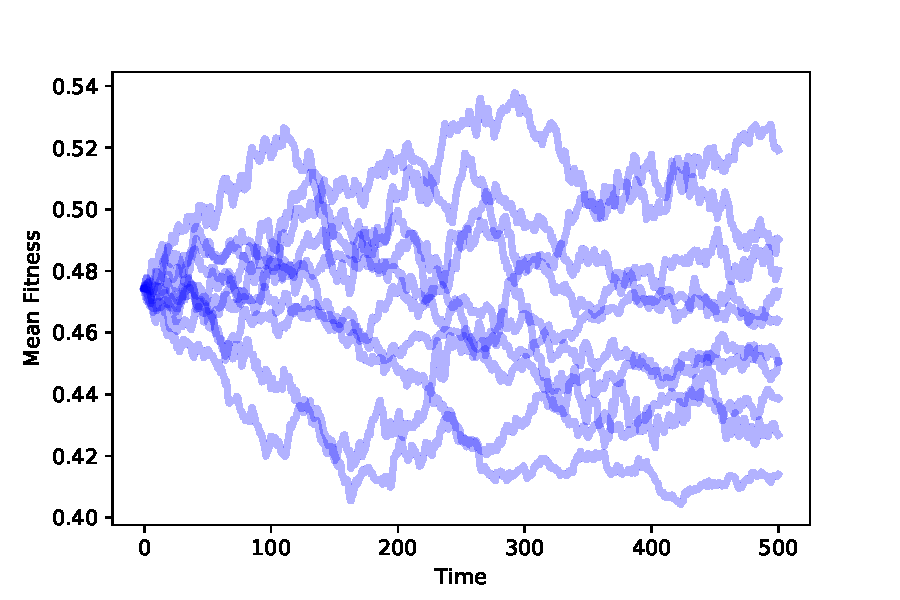
\includegraphics[height=3in]{figs/chap11-1.pdf}}
\caption{Mean fitness over time for 10 simulations with no differential survival or reproduction.}
\label{chap11-1}
\end{figure}

Figure~\ref{chap11-1} shows the results of running this simulation, with the \py{MeanFitness} instrument, 10 times.

The mean fitness of the population drifts up or down, due to chance.  Since the distribution of fitness changes over time, we infer that the distribution of phenotypes is also changing.  By the most inclusive definition, this {\bf random walk} is a kind of evolution.  But it is not a particularly interesting kind.

In particular, this kind of evolution does not explain how biological species change over time, or how new species appear.  The theory of evolution is powerful because it explains phenomena we see in the natural world that seem inexplicable:

\begin{itemize}

\item Adaptation: Species interact with their environments in ways that seem too complex, too intricate, and too clever to happen by chance.  Many features of natural systems seem as if they were designed.

\item Increasing diversity: Over time the number of species on earth has generally increased (despite several periods of mass extinction).

\item Increasing complexity: The history of life on earth starts with relatively simple life forms, with more complex organisms appearing later in the geological record.

\end{itemize}

These are the phenomena we want to explain.  So far, our model doesn't do the job.


\section{Differential survival}

So let's add one more ingredient, differential survival.  Here's the definition for a class that extends \py{Simulation} and overrides \py{choose_dead}:

\begin{code}
class SimWithDiffSurvival(Simulation):
    
    def choose_dead(self, fits):
        n = len(self.agents)
        is_dead = np.random.random(n) > fits
        index_dead = np.nonzero(is_dead)[0]
        return index_dead
\end{code}

Now the probability of survival depends on fitness; in fact, in this version, the probability that an agent survives each time step {\em is} its fitness.

Since agents with low fitness are more likely to die, agents with high fitness are more likely to survive long enough to reproduce.  So we expect the number of low-fitness agents to decrease, and the number of high-fitness agents to increase.  If we plot the mean fitness over time, we expect it to increase.

\begin{figure}
\centerline{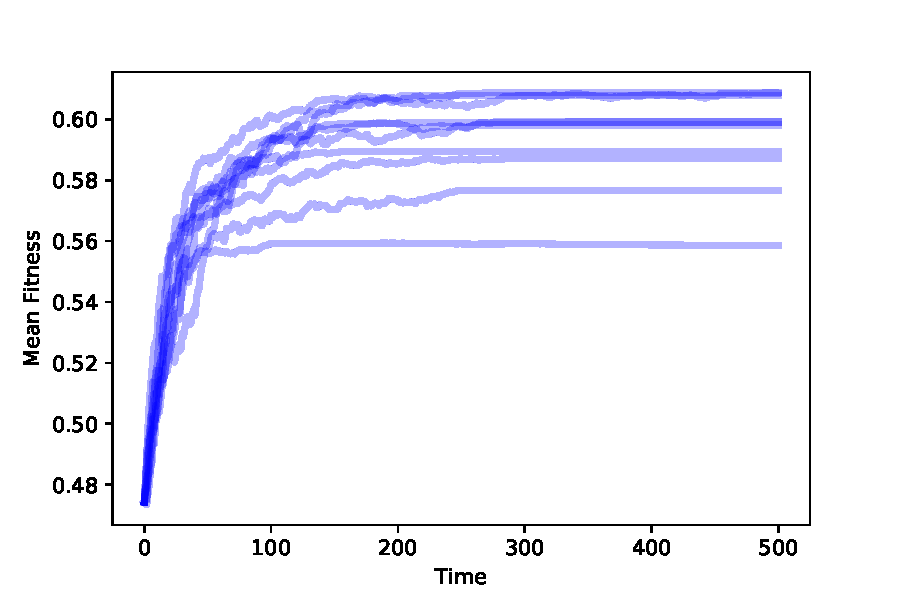
\includegraphics[height=3in]{figs/chap11-2.pdf}}
\caption{Mean fitness over time for 10 simulations with differential survival.}
\label{chap11-2}
\end{figure}

Figure~\ref{chap11-2} shows the results of 10 simulations with differential survival.  Mean fitness increases quickly at first, but then levels off.

You can probably figure out why it levels off: if there is only one agent at a particular location and it dies, it leaves that location unoccupied.  And without mutation, there is no way for it to be occupied again.

With \py{N=8}, this simulation starts with 256 agents occupying all possible locations.  Over time, the number of unique locations decreases; if the simulation runs long enough, eventually all agents will occupy the same location.

So this simulation starts to explain adaptation: increasing fitness means that the species is getting better at surviving in its environment.  But with a decreasing number of locations, it does not explain increasing diversity at all.

In the notebook for this chapter, you will see the effect of differential reproduction.  As you might expect, differential reproduction also increases mean fitness.  But without mutation, we still don't see increasing diversity.

\section{Mutation}

In the simulations so far, we start with the maximum possible diversity --- one agent at every location in the landscape --- and end (eventually) with the minimum possible diversity, all agents at one location.

That's almost the opposite of what happened in the natural world, which apparently began with a single species that branched, over time, into the millions, or possibly billions, of species on Earth today (see \url{https://en.wikipedia.org/wiki/Global_biodiversity}).

With perfect copying in our model, we never see increasing diversity.  But if we add mutation, along with differential survival and reproduction, we get a step closer to understanding evolution in nature.

Here is a class definition that extends \py{Agent} and overrides \py{copy}:

\begin{code}
class Mutant(Agent):
    
    prob_mutate = 0.05
    
    def copy(self):
        if np.random.random() > self.prob_mutate:
            loc = self.loc.copy()
        else:
            direction = np.random.randint(self.fit_land.N)
            loc = self.mutate(direction)
        return Mutant(loc, self.fit_land)
\end{code}

In this model of mutation, every time we call \py{copy}, there is a 5\% chance of mutation.  In case of mutation, we choose a random direction from the current location --- that is, a random bit in the genotype --- and flip it.  Here's \py{mutate}:

\begin{code}
    def mutate(self, direction):
        new_loc = self.loc.copy()
        new_loc[direction] ^= 1
        return new_loc
\end{code}

Now that we have mutation, we don't have to start with an agent at every location.  Instead, we can start with the minimum variability: all agents at the same location.

\begin{figure}
\centerline{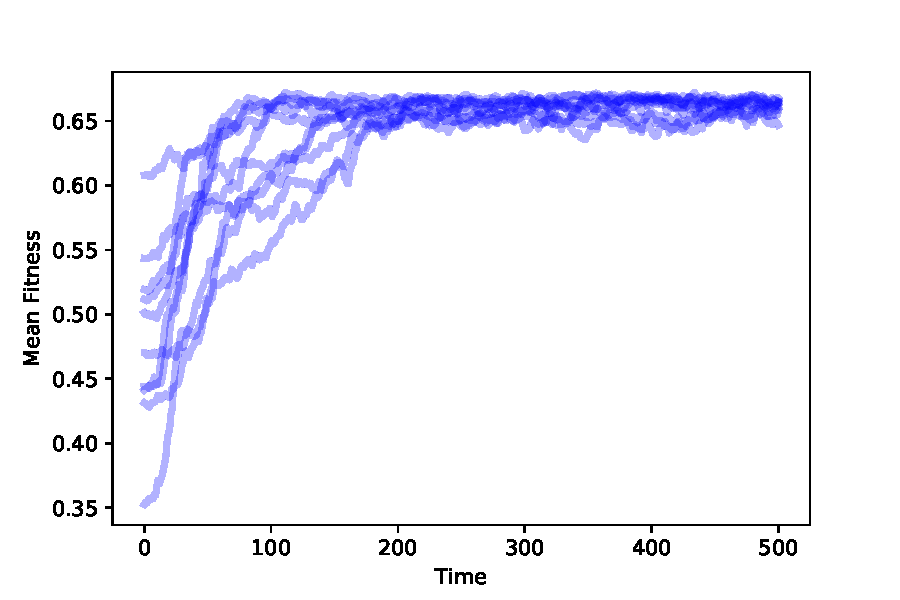
\includegraphics[height=3in]{figs/chap11-3.pdf}}
\caption{Mean fitness over time for 10 simulations with mutation and differential survival and reproduction.}
\label{chap11-3}
\end{figure}

Figure~\ref{chap11-3} shows the results of 10 simulations with mutation and differential survival and reproduction.  In every case, the population evolves toward the location with maximum fitness.

\begin{figure}
\centerline{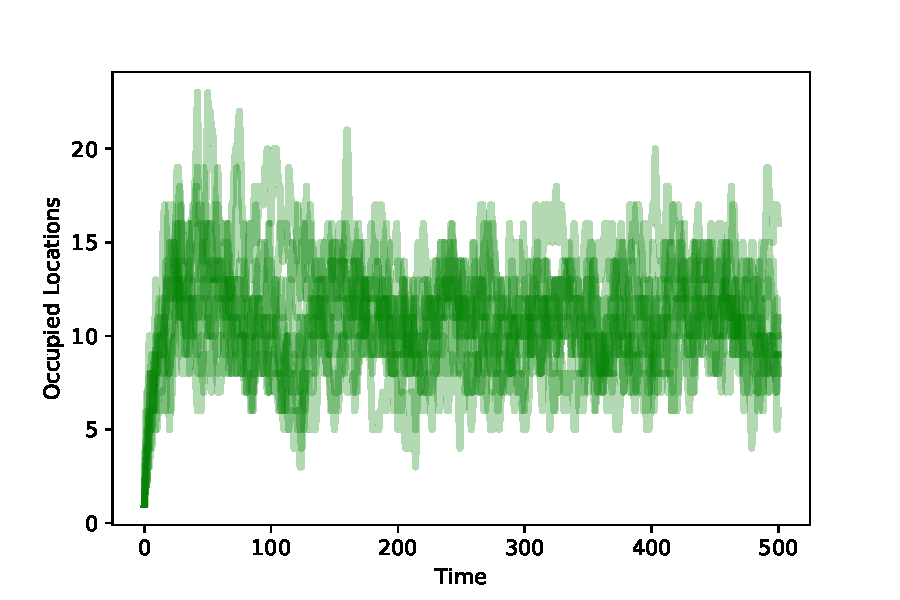
\includegraphics[height=3in]{figs/chap11-4.pdf}}
\caption{Number of occupied locations over time for 10 simulations with mutation and differential survival and reproduction.}
\label{chap11-4}
\end{figure}

To measure diversity in the population, we can plot the number of occupied locations after each timestep.  Figure~\ref{chap11-4} shows the results.  We start with 100 agents, all at the same location.  As mutations occur, the number of occupied locations increases quickly. 

When an agent discovers a high-fitness location, it is more likely to survive and reproduce.  Agents at lower-fitness locations eventually die out.  Over time, the population migrates through the landscape until most agents are at the location with the highest fitness.

At that point, the system reaches an equilibrium where mutation occupies new locations at the same rate that differential survival causes lower-fitness locations to be left empty.

The number of occupied locations in equilibrium depends on the mutation rate and the degree of differential survival.  In these simulations the number of unique occupied locations at any point is typically 5--15.

It is important to remember that the agents in this model don't move, just as the genotype of an organism doesn't change.  When an agent dies, it can leave a location unoccupied.  And when a mutation occurs, it can occupy a new location.

As agents disappear from some locations and appear in others, the population migrates across the landscape, like a glider in Game of Life.  But organisms don't evolve; populations do.


\section{Speciation}

The theory of evolution says that natural selection changes existing species and creates new ones.  In our model, we have seen changes, but we have not seen a new species.  It's not even clear, in the model, what a new species would look like.

Among species that reproduce sexually, two organisms are considered the same species if they can breed and produce fertile offspring.  But the agents in the model don't reproduce sexually, so this definition doesn't apply.

Among organisms that reproduce asexually, like bacteria, the definition of species is not as clear-cut.  Generally, a population is considered a species if their genotypes form a cluster, that is, if the genetic differences within the population are small compared to the differences between populations.

\begin{figure}
\centerline{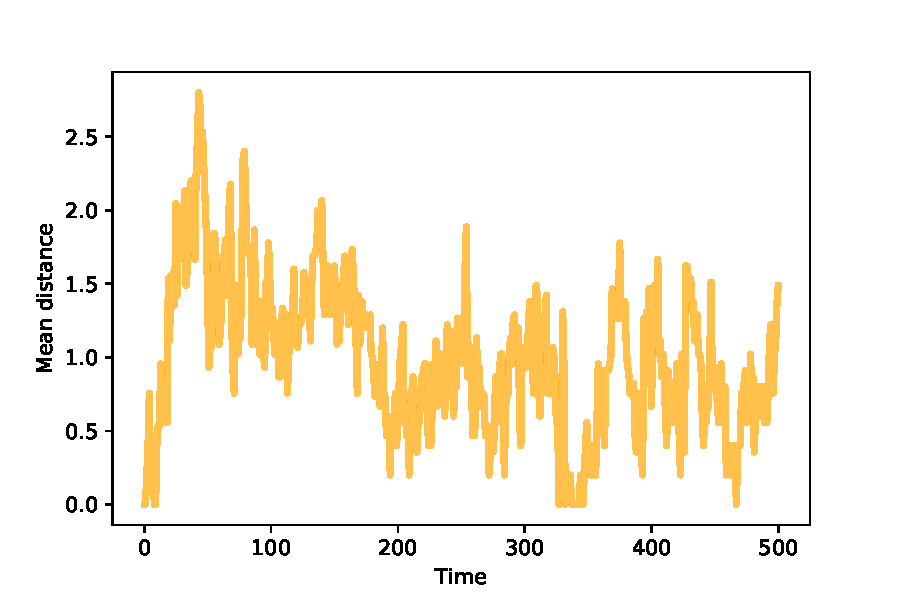
\includegraphics[height=3in]{figs/chap11-5.pdf}}
\caption{Mean distance between agents over time.}
\label{chap11-5}
\end{figure}

So before we can model new species, we need the ability to identify clusters of agents in the landscape, which means we need a definition of {\bf distance} between locations.  Since locations are represented with strings of binary digits, we'll define distance as the number of bit in the genotype that differ.  \py{FitnessLandscape} provides a \py{distance} method:

\begin{code}
# class FitnessLandscape

    def distance(self, loc1, loc2):
        return np.sum(np.logical_xor(loc1, loc2))
\end{code}

The \py{logical_xor} function is \py{True} for the elements of the locations that differ, and \py{False} for the elements that are the same.

To quantify the dispersion of a population, we can compute the mean of the distances between every pair of agents.  In the notebook for this chapter, you'll see the \py{MeanDistance} instrument, which computes this metric after each time step.

Figure~\ref{chap11-5} shows mean distance between agents over time.  Because we start with identical mutants, the initial distances are 0.  As mutations occur, mean distance increases, reaching a maximum while the population migrates across the landscape.

Once the agents discover the optimal location, mean distance decreases until the population reaches an equilibrium where increasing distance due to mutation is balanced by decreasing distance as agents far from the optimal location are more likely to die.  In these simulations, the mean distance in equilibrium is near 1.5; that is, most agents are only 1--2 mutations away from optimal.

Now we are ready to look for new species.  To model a simple kind of speciation, suppose a population evolves in an unchanging environment until it reaches steady state (like some species we find in nature that seem to have changed very little over long periods of time).

Now suppose we either change the environment or transport the population to a new environment.  Some features that increased fitness in the old environment might decrease it in the new environment, and vice versa.

We can model these scenarios by running a simulation until the population reaches steady state, then changing the fitness landscape, and then resuming the simulation until the population reaches steady state again.

\begin{figure}
\centerline{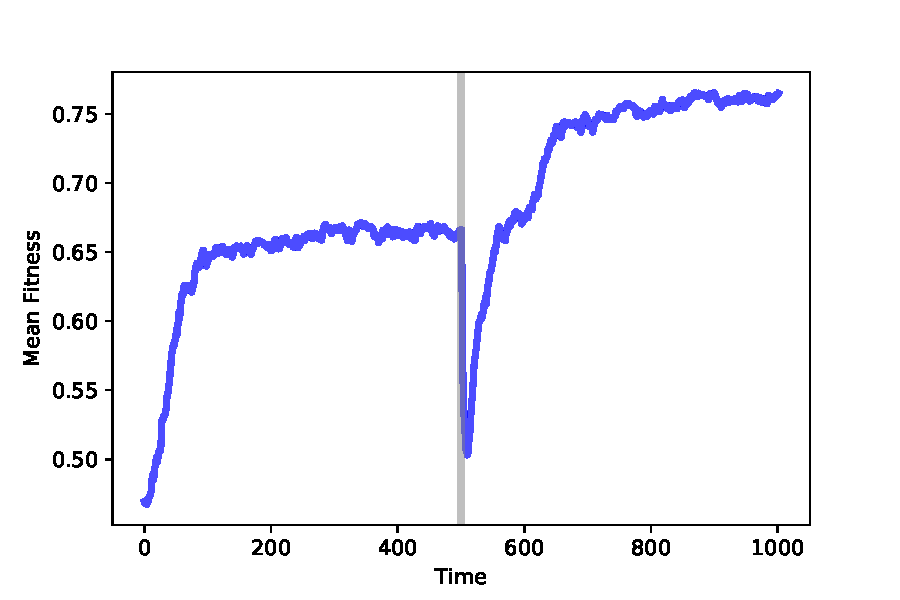
\includegraphics[height=3in]{figs/chap11-6.pdf}}
\caption{Mean fitness over time.  After 500 timesteps, we change the fitness landscape.}
\label{chap11-6}
\end{figure}

Figure~\ref{chap11-6} shows results from a simulation like that.  Again, we start with 100 identical mutants at a random location, and run the simulation for 500 timesteps.  At that point, many agents are at the optimal location, which has fitness near 0.65, in this example.  And the genotypes of the agents form a cluster, with the mean distance between agents near 1.

After 500 steps, we run \py{FitnessLandscape.set_values}, which changes the mapping from genotype to fitness; then we resume the simulation.  Mean fitness drops immediately, because the optimal location and its neighbors in the old landscape are no better than random locations in the new landscape.

However, mean fitness increases quickly as the population migrates across the new landscape, eventually finding the new optimal location, which has fitness near 0.75 (which happens to be higher in this example, but needn't be).

Once the population reaches steady state, it forms a new cluster, with mean distance between agents near 1 again.

Now if we compute the distance between the agents' locations before and after the change, they differ by more than 6, on average.  The distances between clusters are much bigger than the distances between agents in each cluster, so we can interpret these clusters as distinct species. 


\section{Summary}

We have seen that mutation, along with differential survival and reproduction, is sufficient to cause increasing fitness, increasing diversity, and a simple form of speciation.  This model is not meant to be realistic; evolution in natural systems is much more complicated than this.  Rather, it is meant to be a ``sufficiency theorem"; that is, a demonstration that the features of the model are sufficient to produce the behavior we are trying to explain (see \url{https://en.wikipedia.org/wiki/Necessity_and_sufficiency}).

Logically, this ``theorem" doesn't prove that evolution in nature is caused by these mechanisms alone.  But since these mechanisms do appear, in many forms, in biological systems, it is reasonable to think that they at least contribute to natural evolution.

Likewise, the model does not prove that these mechanisms always cause evolution.  But the results we see here turns out to be robust: in almost any model that includes these features --- imperfect replicators, variability, and differential reproduction --- evolution happens.

I hope this observation helps to demystify evolution.  When we look at natural systems, evolution seems complicated.  And because we primarily see the results of evolution, with only glimpses of the process, it can be hard to imagine and sometimes hard to believe.

But in simulation, we can see the whole process, not just the results.  And by including only the minimal set of features to produce evolution --- temporarily ignoring the vast complexity of biological life --- we can see evolution as the surprisingly simple, inevitable idea that it is.

